%%=============================================================================
%% Inleiding
%%=============================================================================

\chapter{Introduction}
\label{ch:inleiding}

The first chapter will introduce the the goal of this paper and will provide the functional and technical content surrounding the research and the proof of concept.

\section{State of the art}
\label{sec:stand-van-zaken}

equensWorldline is with no doubt the biggest player on the Belgian market when it comes to processing electronic card payments.
When someone pays with his or her card, debit or credit, there is a very real chance the transaction will be processed by this company.
Especially for the domestic scheme Bancontact, in nearly all cases the transactions will pass through equensWorldline one way or another \autocite{internal} .
Critical problems on the side of equensWorldline could potentially cripple the Belgian economy, and this is not unseen.
Several years ago there was a critical issue that caused card payments to be down for two hours. This happened on the twenty-third
of December, one of the busiest days of the year for retail \autocite{outage}. 

The pressure for incidents like this not to happen is huge. Several institutions, including the National Bank of Belgium,
watch closely over equensWorldline. After a major incident, extra security measures always have to be taken. One of those measures was to set up an internal plan
to strictly govern critical data in the company. This essential data is spread
across the different IT platforms. Even though the high level guidelines are the same for all systems, every one of them has
a different implementation. One of these platforms is a NonStop machine.

On the NonStop there are two ways of storing critical data. There is Enscribe and there is Nonstop-SQL.
The request has come to create a program to assist in auditting the essential data. A solution has been designed
and developed for the SQL tables, but not for the Enscribe files.


\section{Problems and research}
\label{sec:onderzoeksvragen}

The goal of this research is to create an Enscribe solution to go along with the already established SQL program. To accomplish this we will first identify which
database transactions were used in the SQL version and how they can be implemented for Enscribe. After that, 
the implementations for these requirements will be compared and potential problems will be highlighted. All
this is done to answer the questions:

\begin{itemize}
	\item What is Enscribe?
	\item What are the differences between Enscribe and SQL for this solution?
	\item Can an equivalent solution to the SQL version be implemented for Enscribe?
\end{itemize}

Apart from the official HP-manuals, there is not much information to be found about Enscribe. The research will be conducted by using those official manuals and putting it to work in code. This is why a proof of concept will be made to follow up on the findings. The PoC will use all the conclusions of the research to implement
an Enscribe solution.

This paper makes the assumption that the reader has some basic knowledge about SQL, but is not familiar with Enscribe or file-based database systems.

\section{Structure of the document}
\label{sec:opzet-bachelorproef}


In order to fully understand the functional and technical requirements and context, this paper will zoom in on
on several items before the research. First equensWorldline and the NonStop system will be discussed, followed by the history and problems of databases and database management. This will be chapter~\ref{ch:inleiding}.

Chapter~\ref{ch:methodologie} will describe the research and effort done in order to provide a solution to the aforementioned problems and questions. There is an extensive dive into Enscribe, as this is a technology unique to NonStop and is not widely discussed or researched. 

The proof of concept will be full discussed and described in chapter\ref{ch:poc}.

In Chapter~\ref{ch:conclusie} the paper will conclude the results, answer the questions of the research and discuss what impact this work could have in the future.

\section{equensWorldline}
In the late sixties and seventies, payment by card became increasingly popular
all around the world \autocite{historyMC}. Card payments eliminated a lot risks and introduced many benefits for both the consumer
and the merchants. Not having to carry around a lot of cash, no bad checks or possibility to dispute are all assets
of using a card. Riding this global wave of popularity, several card issuing companies and schemes
like MasterCard and Visa, started globalizing their business \autocite{historyMC}. But not only global players saw their chances to thrive.
A lot of countries and bank unions invested in launching their own domestic scheme such as Cartes Bancaires in France,
Bancomat in Italy and Bancontact here in Belgium. 

Banksys was founded in 1989 by several banks. It had the purpose to enable electronic payments 
in Belgium. Banksys covered full end to end transactions starting at the terminal at the merchant, doing the acquiring and processing
the issuing \autocite{BanksysAtos}. Acquiring and issuing are both 2 important phases in classical card payment. Banksys was sole player on several aspects of the payment chain for
Bancontact until 2006 \autocite{monopoly}, \autocite{intern}. 

Around that time, guidelines were set within the context of SEPA to open up all aspects of electronic payment to
new and other players for all schemes and electronic payment means. SEPA stands for Single Euro Payments Area and is an initiative
by the European Union and European financial institutions to harmonize and standardize all electronic payments across Europe \autocite{SEPA}. In light of these European guidelines, the IT company Atos acquired Banksys. From that point on Banksys was part of the Atos Worldline group.
This is a group of Atos companies that are all active within electronic payments, not only in Europe but all around the world. 
Since then, the Atos Worldline group has not stopped growing. In the meantime a lot more entities have joined and merged with the group.
One of those companies was Equens \autocite{AtosWorldline}. 

A new legal entity was found when the Worldline group acquired Equens. This new entity 
received the name equensWorldline. equensWorldline is the largest payment transaction processing company in Europe \autocite{AtosWorldline}. It processes around
10 billion transactions  per year, and this number is only estimated to increase every year. For Bancontact alone in Belgium,
the rate of transactions can go up to 17.000 per minute on busy days\autocite{hlnrec}. 

equensWorldline is active in almost every aspect of electronic payments. This can be
acquiring, issuing, terminals, e-commerce and a lot more. Especially since the rise of e-commerce in a lot of European
countries, new ways and means of paying electronically have emerged \autocite{ecom}. equensWorldline follows the new trends and  participates in new and innovative ways
of payment. An example of this is the very popular method in The Netherlands called iDeal,
which equensWorldline does all the processing for \autocite{intern}. 

Being a financial institute requires a lot of licenses and approval. These licenses are obtained by complying to security standards set by different institutes.
The National Bank of Belgium is the main regulator here in Belgium. It enforces national and Europeans laws and regulations
on financial institutes \autocite{NBB}. Some of these licenses are also issued by the market leaders and popular schemes in payment. An example of this is the PCI license.
PCI compliance is governed by 5 global players such as Visa and MasterCard \autocite{PCI}. In order to keep these licenses
and thus stay in business, equensWorldline must make sure it keeps up in compliance. Since the core business is IT, a large
part of being complaint relies on the infrastructure and operation procedures. 

\section{HP NonStop}

To handle huge volumes of transactions, there is need for a very stable, reliable and available 
IT infrastructure. As mentioned earlier, equensWorldline partakes in a lot of different aspects regarding
e-payment. These activities are spread out between a variety of different 
systems. Among these systems are Unix servers, an Open-VMS system and a HP-NonStop mainframe. The latter
is the system on which this research is focussed.

\subsection{NonStop}
Nonstop is described by it's current manufacturer Hewlet-Packard Company, or HP, as fault-tolerant server technology. A Nonstop system is
a combination of hardware and software that create a highly available, fault tolerant, high performance and scalable IT solution for businesses.
They are often called main-frame like systems \autocite{hpnonstop}. However, the NonStop machines are vastly different from the classical mainframes, like the ones IBM provides.
Here is the definition of the word mainframe found in the \cite{mainframedef} online dictionary.
\begin{quote}
	A large, powerful computer that can handle many tasks concurrently and is usually used commercially.
\end{quote}

Going by this definition, a NonStop machine are technically a mainframe. However, it is much more than just a large, powerful computer.
The Nonstop should be seen as the entire system and philosphy that come with the hardware and software. 
It is vastly different from the classical mainframes. Other mainframe systems are usually
batch oriented, where scheduling jobs is a very important part. NonStop on the other hand, is all about real-time transaction processing.
Even though batch work is possible, there are usually no queues and processes are just started.

Generally the NonStop machines are used in environments where high availability and large amount of transactions
are the norm. Finance, telecom or retail are prime examples of markets suited for a NonStop machine \autocite{hpnonstop}. Examples in Belgium today
are equensWorldline, Proximus and Euroclear. 

\subsection{History}
The NonStop product line was originally introduced by a company named Tandem Computers. 
The people that started this organisation in 1974, were a group of engineers working at Hewlett-Packard Company or HP. They had the main goal
of designing and manufacturing a system that was safe from a single point of failure and keeping the price
competitive with other non-fault tolerant systems. They accomplished this by using several redundant components
like processors and storage devices in their architecture \autocite{nonstophistory}. Single point of failure and high availability go hand in hand,
and as the name NonStop would suggest, the systems were designed to be highly available and keep running at all times.

The design of the first Tandem system was complete in 1975. The first system could have
anywhere between 2 and 16 processors. Each of those could reach about 0.7 million instructions per minute.
All these processors were equipped with their own memory, I/O channels and inter-CPU connections. Note that 
all paths and channels were always doubled to support cases of single failures. 
Citibank, a large financial institution, was the first client to install a NonStop system in 1976 \autocite{nonstophistory}.

One of the keystones of NonStop was without a doubt the operating system. It was originally named Tandem Operating System 
but was renamed to Guardian shortly after release. The Guardian operating system supports fail-safe transactions meaning that there
is no loss of data when a program fails at any point. Later on, in 1994, a new environment was added to the operating system alongside Guardian \autocite{nonstophistory}.
This new environment called Open System Services, OSS, provided a POSIX compatible environment on the NonStop. 
It was thus no longer mandatory to learn Guardian. Anyone familiar with Unix systems can easily start with 
OSS on NonStop.

Along the years, a lot of different NonStop series and products have been released. Every series was usually 
introduced with new hardware and new versions for the operating system were and are regularly pushed. Also important new software and concepts
were pushed throughout time,
notably TMF in 1983 and NonStop-SQL in 1986. These is discussed further in section~\ref{section:toodoo} and section~\ref{section:toodoo}.
In 1997 Compaq acquired Tandem
Computers \autocite{compaqtandem}. A few years later, in 2001, HP merged with Compaq \autocite{hpcompaq} bringing Tandem Computers right back to their roots.

\subsection{Nonstop Today}

In modern day, mainframes and mainframe-like systems are often coping with an image problem \autocite{imageproblem}.
They are often labelled as old and referred to as dinosaurs. It's hard for companies to find people familiar
with the machines and fresh graduates are often not interested in working with the older technologies \autocite{recruit}.
When companies using a mainframe decide to eliminate the system from their business, this is often a decision made by management who are not
involved in working with the machine and merely see the costs \autocite{imageproblem}.

However, NonStop is still very much relevant and up to date. HP reports an average growth rate of 1.5 in NonStop sales across Europe and America last year,
and a spectacular growth rate of 2.8 in Japan. Although mainframes are often more expensive as alternative solutions, the core strengths are unparalleled.
Amongst these advantages are availability, security and performance \autocite{imageproblem}. 

To stay modern and keep up with modern standards HP has continuously updated and improved their systems. The
latest NonStop machines have migrated from Itanium processors to x86 architecture. The series is named NonStop X. They have also been
eliminating the need for NonStop specific hardware. In the new systems they are opting to use components adhering to market standards. This
implies that the pieces of hardware were not specifically designed for NonStop and can easily be reused by other systems \autocite{presentation}.

Although not available yet, HP is working on virtualized NonStop without the need for any specific hardware.
It will be possible to install it in a cloud or on pre-existing systems. Note that these systems do not have to be HP NonStop servers. They could
even be a Unix server park. This brings a whole new dimension to NonStop. This new product should open up the mainframe market to business that were previously
set back by the size and investment of the classic machines \autocite{presentation}.

\subsection{Nonstop @WL}

This will contain a more technical description of the NonStop machine eWl is using. Awaiting info from the system team. 
\newpage
\section{Databases}
A core concept in IT is data storage. When programs and systems are developed, data storage is one of the key factors to keep in mind. Whether it is just some start up configuration data or huge amounts of data dumps, the right choice in architecture and technologies can make or break the success of projects. 

Especially in environments where transaction speeds and response times are crucial, it is imperative that the database layer does not cause to be a bottle neck. Disk I/O's are usually costly when it comes to CPU time and usage. This means it is not only important that the architecture and technology was chosen right, but also that the approach towards the data is done in an efficient and logical way.

In order to gain some more understanding towards the classic issues and discussions, following section will discuss the history of database systems. 

\subsection{Hardware}

\subsubsection{Punch cards}
\begin{wrapfigure}{r}{0.3\textwidth}
	%	\vspace{-15pt}
	
	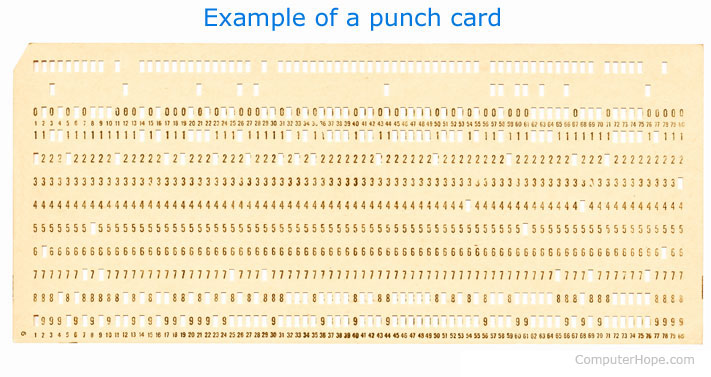
\includegraphics[scale=0.22]{punch-card} 
	\caption{Punchcard \autocite{punch}}
	\label{fig:punchcard}
	%	\vspace{-20pt}
\end{wrapfigure}
One of the most iconic methods to store data, is without a doubt the classic Punch cards. They were paper slips that would be perforated in order to store data. Every column would present a character, and the rows were punched to indicate it's value. One card would contain about 80 characters, around 960 bits of data. For example, to store the picture~\ref{fig:punchcard}, showing a punch card, one would need 655 cards. They would also have to be kept in order, or the data would not make any more sense. It is clear that this way of working is very error prone, boorish and inefficient. The first use reported of punch cards dates as far back as 1725 and were mostly all replaced in the sixties \autocite{punch}.

\subsubsection{Tapes}
Following the punch cards were tapes. They were introduced in the early fifties and found a lot of success on the market \autocite{tape}. Tapes are a lot more reliable and faster than the previous solutions thus far. They can even be encrypted! There were however still some setbacks. When the tape gets to it's end, it had to be replaced. The access to the tape was, just like the punch cards, sequential only. So if you need some data that is in the middle of your tape, you would have to scan at least all the data coming before your wanted piece. 

\subsubsection{Hard Drives}
In the same era, in 1957, hard disk drives saw it's first commercial use \cite{hdd}. They introduced the ability to randomly access data. The fact that data did not have to be accessed sequential any more was huge. This led to a huge increase in speed of data access \autocite{hdd}. Naturally, the cost was a lot higher than tapes. A common solution was and is to have all the critical data on hard drives, and use the cheaper solutions for back ups.

 Since then data devices have only improved and new technologies have sprouted since. Floppy's, CD's or SSD's are just some examples of popular inventions that are no longer bound by sequential access. 
 
\subsection{File systems}
The traditional file based approach is the predecessor of the modern day database management systems. Although they are not, and should not, be used for commercial applications any more, they still define the base concepts for some technologies. There is much to learn from these systems as to how we should and should not handle data.

These systems work by placing data into a file. These files contain data. Each line can be associated with a record and contains data. These files can then be moved into their corresponding folder. For example: students in a class. The records in the file would be the information about the students. This file would define a collection of them, containing all those enrolled. It could then be placed in the folder of the class it belongs to, which in its turn is placed in the school folder. This concept is the baseline for the file-based approach and it is called a hierarchical structure. 

	\begin{center}
		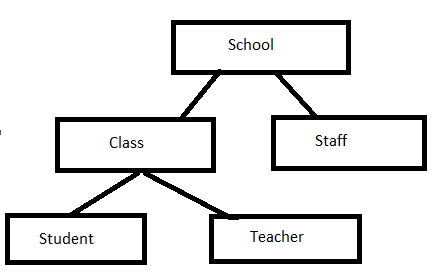
\includegraphics[scale=0.45]{file-structure} 
		\captionof{figure}{Hierarchical structure}
	\end{center}

Even though this approach sounds every logical and reasonable, there are limitations and problems. To illustrate these, the example in the paragraph just above will serve as illustration applied to the issues documented by \cite{dbhist1}.

\subsubsection{Separation and isolation of data}
It can be hard and obfuscated to find fairly simple requests. Say the principal of the school would like to know how many children in his school live within a certain range. He would then have to navigate through all the classes to list all the children. The information is further away than it needs to. Processing the information becomes unnecessarily complicated.

\subsubsection{Duplication of data}
Some data is stored more than once. If a teacher moves to a new home, his address will have to be changed. However one department uses the staff file to process payments, while the scheduling team also has a collection of teachers linked to the classes. This change in address would have to be communicated to both departments. It is clear that this is a waste of resources and is very error prone. If a mistake is made in one of the files, the data is no longer consistent.

\subsubsection{Data dependence}
In a system like this, which has no data managing layer, it is the applications themselves who are responsible for defining what the data is they receive. Say the school wants to add a field in the student records, that define they can leave school during lunch. All the programs that work with the student file will have to be adjusted in order for the system to keep working. This can create an immense overhead for what was intended to just be a small change.

\subsubsection{Incompatible file format}
The technology used to create applications for the school, has to support the used file format. Different programming language can possibly generate different structures, making the files incompatible. This would imply that all the departments have aligned IT solutions and this again, can create an unnecessary overhead.

\subsubsection{Application responsibility}
All the responsibility of handling the data is on the application. Not only structure wise, but also query wise. If new questions rise from the business side that can not be answered with an existing functionality in the program, it would need a programmer to revisit the application and code the new logic into the program. Again, this is creating extra work and requires unnecessary effort.

\subsubsection{Poor concurrent user management}
Checking for locks, making sure it is safe to update or having the latest version of file are all responsibilities for the application. There is no overseeing instance that can guarantee no other program is using the files for processing or updating. This causes a threat to the data integrity of the system. 

\subsection{Database Management Systems}
It is clear that the hierarchical approach to mapping and storing data is not ideal. It is not open to change, it can create a lot of unneeded and unwanted work, it can be very obfuscated and it can lead to breach of data integrity. Several vendors brought technologies on the market attempting to tackle the issues of a classical file based approach \autocite{dbhist2}.

\cite{dbhist1} defines a database management system, or DBMS, as:
\begin{quote}
	A software system that enables users to define, create, maintain, and control
	access to the database.
\end{quote}

Discuss the working of DBMS, mention different brands, mention relatianal mention it can be on top of files/relational and variety of advantages and disadvantages


\subsection{NonStop SQL}

Small section about the important differences between standard and nonstop SQL

